\chapter{Convolutional Neural Networks}\label{ch_cnn}
\chapterauthor{Jeff Yoshimi, Pierre Beckmann}{.7,.3}


% Discuss deep fakes and GANs?
% Illustrates a standard workflow https://github.com/google-research/tuning_playbook
% Improve discussion of location invariance
% Bias of a layer
% Think of filter banks and pooling layers as the two main analogues of a weight layer in a standard nn.

Convolutional neural networks are a prominent type of deep network. They are a kind of many-layered network that is often used for processing visual inputs, like recognizing patterns in images or movies, though they have broader application. They make use of a special kind of mapping between node layers, a convolutional layer. Before we get into the details, we start with some background motivation.
% Relate terms CNN, deep network, and deep learning 

The idea of re-mapping an input space to a hidden unit space in order to solve classification and regression problems is what drew neural networks out of its first ``dark age'' and back into the limelight, giving rise to an explosion of interest in neural networks in the 1980s and 1990s (chapter \extref{ch_history}). The internal representations of these networks--usually 3 node-layer networks trained by backprop--allowed them to solve previously unsolvable problems like XOR (figure \extref{xor_remapping}). These representations were often psychologically realistic (section \extref{ch_representations}). However, recall that a second  winter lay in wait, as machine learning models became more prominent in the late 1990s and 2000s. What got us out of that second winter was \glossary{deep network}s, that is, networks with more than 3 node layers, trained using new tricks and techniques, like convolutional layers, the use of graphical processing units for fast parallel computation, and the Relu activation function discussed in chapter \extref{ch_act_functions}. These advances made it possible to use the same types network discussed in chapter \extref{ch_lms_backprop} on much more difficult problems.\footnote{This history is well told by Kurenkov in section 3 of \url{https://www.skynettoday.com/overviews/neural-net-history}. As he summarizes, ``Deep Learning = Lots of training data + Parallel Computation + Scalable, smart algorithms.''}  They also developed psychological and neurally realistic internal representations, and thus these networks are of considerable interest across the different domains of neural network research.

In terms of engineering, these convolutional networks have been associated with improvements in image recognition, speech recognition, language translation, and in many other areas \cite{lecun2015deep, goodfellow2016deep}. They do this by creating hierarchies of representations, corresponding  to increasingly complex features of an input image. As we saw in chapter \extref{ch_neuro} (see figure \extref{deepLearning_Vision}) when such networks are trained to recognize images they develop internal representation that are extremely similar to those developed by the human visual  system. Thus they are relevant both to neuroscience (where they can describe the behavior of neurons in the visual system), and to psychology (where they can describe internal representations humans might rely on).
% More on engineering advances. The nature paper (lecun2015deep) has some helpful information at "first major application"

The topic of deep networks and deep learning are quite involved and the field is active and continues to grow (this is a preliminary chapter on the topic; it will be expanded in the future). Here we will describe some of the main concepts and some of their applications to neuroscience and psychology.

\section{Convolutional Layers}\label{convolutionalLayer}

% Terminology: source layer, source image, pixel array, input volume, output volume

The key idea with a deep network is to use a special type of weight layer called a \glossary{convolutional layer} to efficiently learn to recognize features in a previous layer.\footnote{An outstanding visual discussion of the concept of a convolutions is at \url{https://youtu.be/KuXjwB4LzSA}} Until now we've been dealing with weight layers that connect all the nodes in a source layer to all the nodes in a target layer; these are sometimes called ``dense layers'' or ``fully connected'' layers to contrast them with convolutional layers. By contrast, convolutional layers involve a set of weights that are ``scanned'' or ``passed'' over the source layer's activations to produce activations in a target layer. This can also be called a ``convolution'' of the source layer activations. Networks that feature convolutional layers are called ``convolutional neural networks'' or ``CNNs'' on analogy to ANN for artificial neural network and RNN for recursive neural network.
% Footnote on the mathematical definition of convolution, and how from that standpoint the source node activations are a function from index entries to activations.

\begin{figure}[h]
\centering
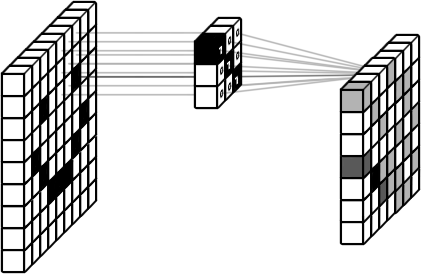
\includegraphics[width=0.5\textwidth]{images/happyConvolution.png}
\caption[Soraya Boza, adapting this image from User Cecbur, \url{https://commons.wikimedia.org/wiki/File:Convolutional_Neural_Network_NeuralNetworkFilter.gif}, with labels added by Jeff Yoshimi.]{A convolutional layer and its components. From left to right: an input image, a 3x3 convolutional filter (which detects edges with a $-45^\circ$ angle), and the resulting feature map. The filter is scanned across the image. At each stage of this scanning process, the dot product of the filter's receptive field in the input image is computed and used to populate the feature map. This whole process is known as a convolution and a layer like this is a convolutional layer.}
\label{cnn_filter}
\end{figure}

\begin{figure}[h]
\centering
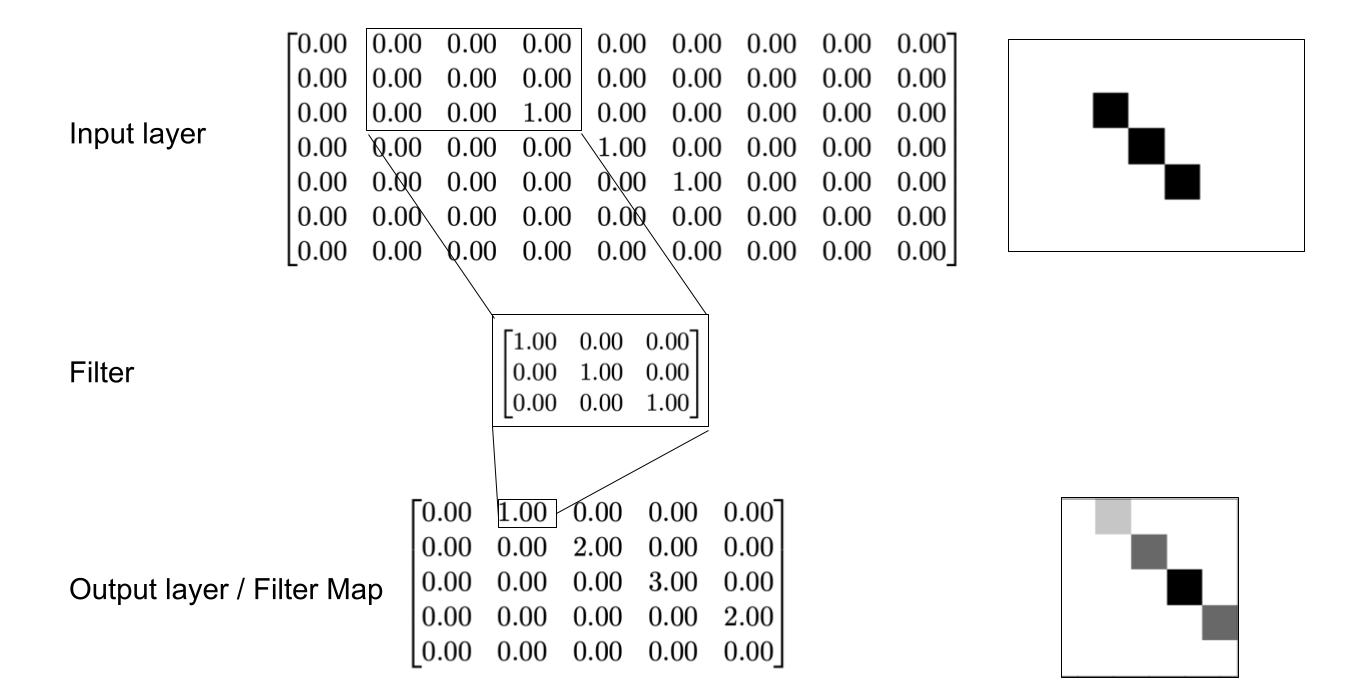
\includegraphics[width=0.7\textwidth]{images/CNN_WorkedExample.png}
\caption[Jeff Yoshimi]{Worked example of a convolutional layer. Notice that the feature map has the highest values where the filter matches the pixel array. In the case shown, the filter matches the pixel array in one pixel only. Imagine the filter sliding over the pixel array, and computing dot products (here: numbers of matching $1$'s), which are used to populate the feature map.}
\label{cnn_workedExample}
\end{figure}

% Expand on weight sharing and add glossary item. Discuss the fact that this is not neurally realistic and ways to understand that.
The weights in a convolutional layer are called a \glossary{filter} or \textbf{kernel}. The weights in a filter are scanned over the source layer to produce outputs. This is a new idea. Rather than a fixed set of weights in a fully-connected weight layer, we have a small set of weights that are reused or shared during the scanning operation (this is also known as ``weight sharing'').

 The source layer of a convolutional layer is often itself a 2d array, prototypically an input image, and so we can think of source layer activations as pixels and the source layer as a pixel array or input volume (even when the input is not an image this language is useful). Filters are like small pixel patterns that we slide across the whole pixel array, which ``light up'' most when they are on top of a similar pixel pattern. The filter is generally moved from left to right and top to bottom of the pixel array. At each stage of the scanning operation, it is multiplied by the patch or ``receptive field''  of the pixel array it is on top of.\footnote{To get a better feel for how this works videos are helpful. A good place  to start is with the first animated gif here: \url{https://stanford.edu/~shervine/teaching/cs-230/cheatsheet-convolutional-neural-networks} This video is also great: \url{https://youtu.be/KuXjwB4LzSA}.} The multiplication is a dot product (see chapter \extref{ch_linear_algebra}), where each weight in the filter is multiplied by the corresponding activation of the pixel array, and the results are added together. Recall that the dot product computes something like a similarity score: the more the filter and the pixels match, the greater the dot product will be. The resulting scalar is used to populate one activation in the target layer. Thus, the convolutional layer computes a kind of \emph{sliding dot product} with the source activations, which highlights where the filter matches the pixel array.
 
 The number of pixels the filter moves at each step is called the \glossary{stride}. Strides can be different in different directions, but we will assume they are the same in all directions. One issue that comes up is the edges, which the filter can't be passed over. To handle this, \glossary{padding} can be added to the input volume, in the form of extra zeros around the edges of the input pixel array. This can be done in such a way that the output volume ends up having the same shape as the input volume (more on this below).\footnote{This page contains an interactive tool that can be used to understand these concepts: \url{https://distill.pub/2019/computing-receptive-fields/}.}

% Reference
In practice, convolutional layers operate on a set of matrices  (an input ``volume'') or a batch of these volumes (a 3d or 4d array; see section \extref{sect_tensors}). The output is often also a volume or batch of volumes. How filters work on volumes is discussed below; we start with the simple case where the input and output of the convolutional layer are matrices, which, again, we refer to as a pixel array and feature map.

The idea is illustrated in figures \ref{cnn_filter} and \ref{cnn_workedExample}. In this example all the numbers are included so you can easily check how the computations are done. A $3 \times 3$ filter is passed over a pixel array, from left to right and top to bottom. At each moment during this scanning process the dot product is computed between the filter and its receptive field in the source matrix (the part of the image the filter is on top of). Since the input image and the filter are both binary, the dot product simply counts how many places the filter overlaps its receptive field as it is scanned over the image. In the example shown, it overlaps in one place, in the bottom right of the filter. So that entry in the target layer is populated with a $1$. Notice that this filter produces the highest value of $3$ only when it is directly on top of the line in the source layer. Try to understand how all the target layer activations are computed. You can also imagine what would happen if the filter or the image were changed.

The output of a convolutional layer is called a \glossary{feature map}. In these examples, the filter is an edge detector, that detects edges at a $-45^\circ$ angle, that is, edges shaped like a backslash `\textbackslash'. In the resulting feature map, notice that the activation is highest when the filter is directly on top of the backslash shape in the happy face, but also produces some activation wherever it is on top of any kind of active pixel. Thus, the feature map gives a sense of where this kind of edge occurs in the input image. \footnote{The code used to generate figure \ref{cnn_workedExample} is available online, and can be used to edit a small filter and kernel to get a feel for how they produce a feature map. See: \url{https://colab.research.google.com/drive/1ywr3z8HRXYNPK-vd34kAATUPVWwwFqQE?usp=sharing}.}

Again, this is totally different from the weight layers we have been studying throughout the book: there are no fixed connections at all. Instead it is like there is a little floating scanner that gets passed over source layer activations to produce output activations. 

There is a performance advantage to these convolutional layers, thanks to the weight sharing. All that must be trained is (in the example shown in figure \ref{cnn_filter}) $3 \times 3=9$ weights, rather than the $81 \times 49 = 3969$ weights that would be required in a fully connected dense layer from the input layer to the feature map. This is a huge performance gain and part of what  made it possible with deep learning to train such large networks.

In general, filters--like this edge detector--are not programmed. This is a neural network after all, and neural networks are trained, not programmed (section \extref{intro_comp_nn}), usually using a form of gradient descent (section \extref{sect_gradient_descent}). Networks trained on vision tasks do not need to be told that edge detectors are useful in early stages of processing. They simply emerge as a structure that supports pattern classification when training a network.

\section{Applying a Filter to a Volume}

So far we have considered an artificial example where the input, filter, and feature map were matrices. However, the power of CNNs is that can deal well with more complex tensors. In the context of image processing (and in most applications of convolutional networks), the input is a volume, a set of multiple stacked matrices or channels, a rank 3 tensor or 3d array. 

To get an initial feel for this situation, think of the filter as a set of filters, one ``sub-filter'' (my term) for each input channel. This set of filters is ``combed'' across the input volume, in the sense that each sub-filter is convolved with a corresponding input channel, and the results are then added together and used to populate one entry in the output matrix. That is how the convolution works. Figure \ref{filterComb} gives a sense of how it works. Convince yourself that the shapes make sense.

\begin{figure}
\centering
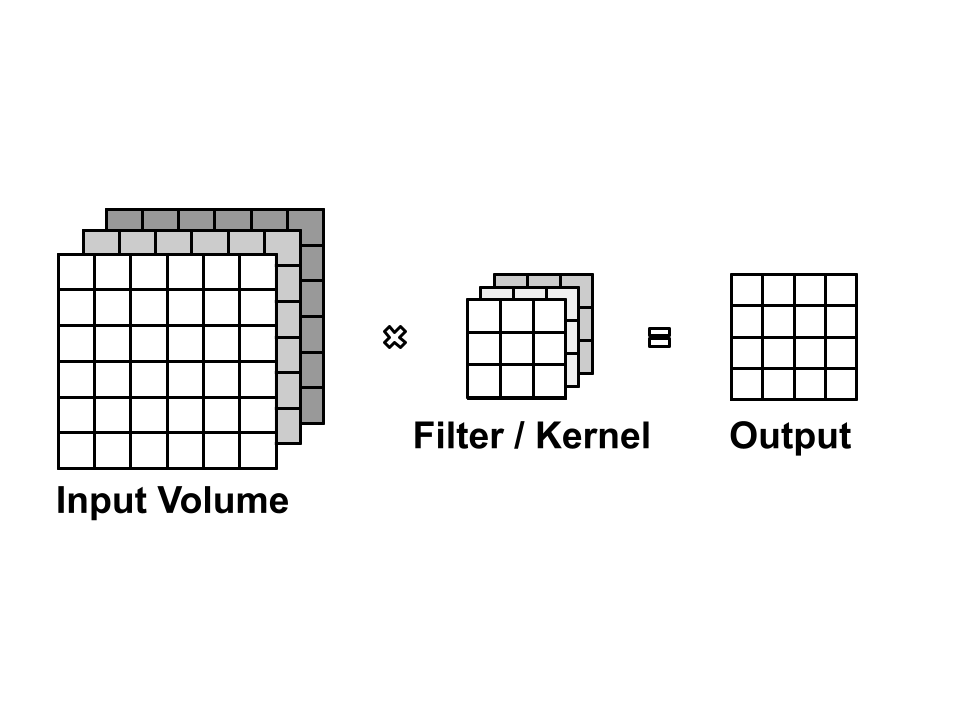
\includegraphics[width=0.5\textwidth]{images/filterComb.png}
\caption[Soraya Boza.]{Applying a filter to an input volume. On the left is an input volume, in the middle is a filter (which includes three sub-filters) and on the right is the output volume that results from convolving or ``combing'' the filter over the input. Each sub-filter is convolved with each input channel, and the results are added together at each stage of the convolution. }
\label{filterComb}
\end{figure}

% Not sure I like this anymore: In a sense this is like a many-to-one connection in a regular neural network. Many nodes connect to one node via a set of weights. Each weight is multiplied by a different input activation and the results are added up to produce a net input. Here instead we have a set of sub-filters, each of which is convolved with one channel in an input volume, and the results are added together.: Reference to net input. If used, could show an actual parallel picture of a 3-1 simbrain net. However the analogy breaks down in the many-to-many case.

But the ``combing'' idea in figure \ref{filterComb} is just a way to ease you into thinking about how convolutions work in practice. Instead of thinking about sets of filters, we can think about filters as volumes which act on other volumes, as in figure \ref{filterToVolume}. That is, we can collapse the ``sub-filters'' of a filter into a single volume, a little Rubik's cube type of object, that convolved with the input as follow. We imagine moving the filter ``through'' the input volume, top-to-bottom and left-to-right, and at each stage of this operation we dot the filter with the receptive field it is on top of. At each stage of this operation the 27 cuboids in the filter are dotted with 27 components of the input volume, and all 27 products are added together. That gives us one entry in the output, which in this simple example is a matrix.

\begin{figure}
\centering
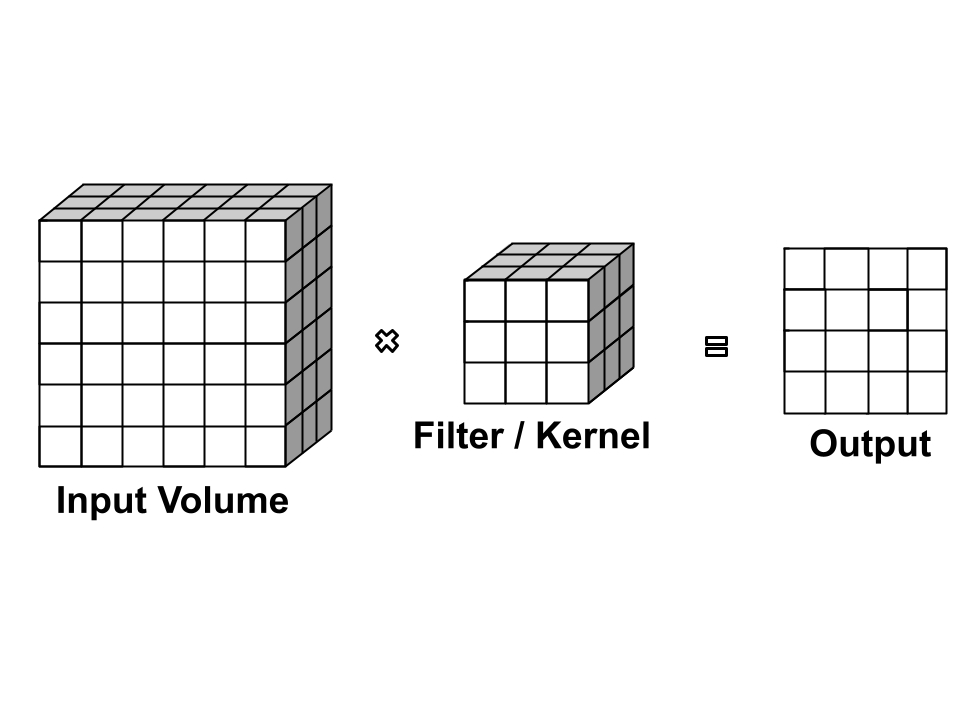
\includegraphics[width=0.5\textwidth]{images/filterToVolume.png}
\caption[Soraya Boza and Jeff Yoshimi.]{The same situation as in figure \ref{filterComb} but represented using volumes. This is a better way to think about convolutional layers, because it generalizes to the more complex situations discussed below. Try to image the filter being passed ``through'' the input volume, and being dotted with its receptive field at each stage of the operation, producing one number in the output.}
\label{filterToVolume}
\end{figure}

In general, the depth of the filter (in the sense of tensor dimensions of depth, width, and height: see section \ref{sect_tensors}) matches the depth of the input volume. That way the filter can capture information from across all the channels. (This is not always shown in figures and can be quite confusing!)  In this example both are of depth 3.\footnote{This is not a necessary feature (filters with fewer channels than the input are possible and sometimes even useful), but it is pretty standard.} Figure \ref{filterDepth} makes the point with a variety of tensors. In each case the receptive field of a filter at one stage of a convolution is shown ``inside'' the input volume, and as can be seen in each case it spans the whole depth of the input. 
% Pierre you mentioned applications with "sculptures" here

\begin{figure}
\centering
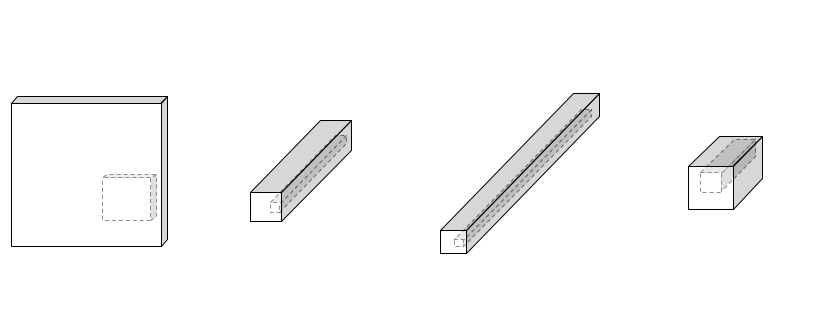
\includegraphics[width=0.9\textwidth]{images/filterDepth}
\caption[Soraya Boza.]{Illustration of how filters must have a depth that matches the input volume they are passed over. Shown is the receptive field of a filter at one stage of a convolutional pass. Alternatively, think of this as the filter itself being placed ``inside'' the input volume and moved through it.}
\label{filterDepth}
\end{figure}

Ignoring padding, the formula for width and height of the output tensor relative to input tensor and filter is:
\begin{align*}
\text{Output Width} &= \left( \frac{\text{Input Width} - \text{Filter Width}}{\text{Stride}} \right) + 1 \\
\text{Output Height} &= \left(  \frac{\text{Input Height} - \text{Filter Height}}{\text{Stride}} \right) + 1
\end{align*}

In the example shown in figures \ref{filterComb} and \ref{filterToVolume} the input width is $6$, the filter width is $3$, and the stride (the amount it is moved for each step of a convolution) is $1$ so the output width is $((6-3)/1 + 1) = 4$. Same for the height. 

The depth of the output shape corresponds to the number of filters we have (more on this soon), and so far we have just considered a single filter, a single ``Rubik's cube''. So the output shape so far in our example is 1. 

So the overall shape of the output is $4 \times 4$, a four-by-four matrix.

\section{Filter Banks (Representational Width)}

% More on representational width. Link to transformers and multi-head attention

In general a convolutional layer will involve multiple filters, a \glossary{filter bank}, each of which produces a separate feature map.  Figure \ref{filterBank} illustrates the idea. Each filter produces its own output, and the results are concatenated into a new output volume. That is, we just repeat the process discussed in figure \ref{filterToVolume} but do it separately for each filter. In this example, we get a bunch of matrix outputs, and concatenate them into one output volume. That is why we said at the end of the last section that the depth of an output volume just corresponds to the number of filters we use. 

\begin{figure}
\centering
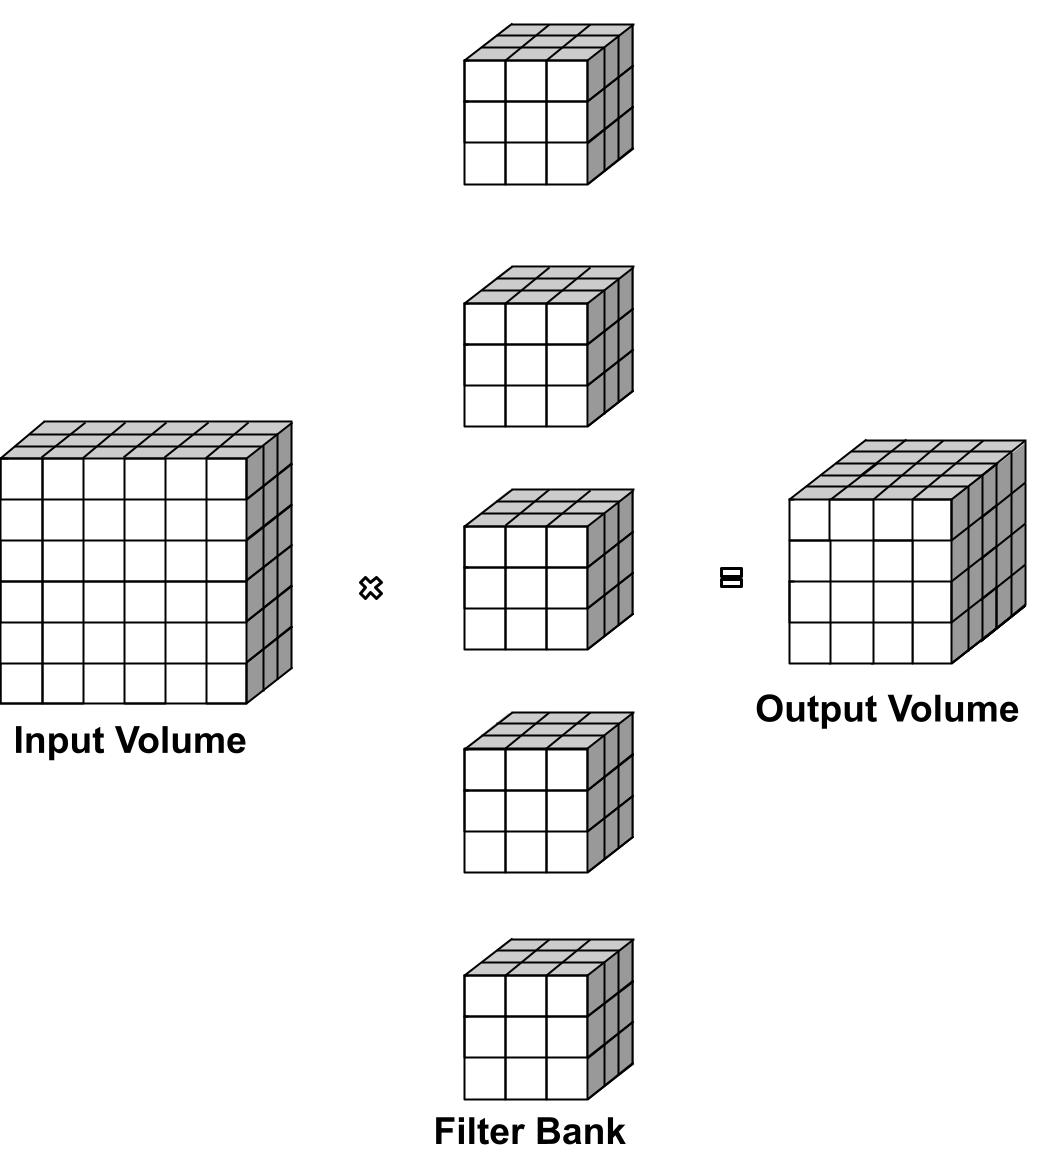
\includegraphics[width=0.5\textwidth]{images/filterBank}
\caption[Soraya Boza and Jeff Yoshimi.]{Result of applying a filter bank of 5 $3 \times 3 \times 3$ filters to a $6 \times 6 \times 3$ input volume to produce an output volume that is $4 \times 4 \times 5$. The height and width come from the formula in the main text, and the depth of $5$ just comes from the number of filters in the bank.}
\label{filterBank}
\end{figure}

Each feature map in a filter bank learns differently via gradient descent to represent the input. Thus we get different ways of representing the input. This generalizes the concept of the \glossary{representational width} of a layer (section \extref{structureNets}) to CNNs. Just as more nodes makes a regular node layer of a feed-forward network more powerful, so too do more filters make a convolutional layer more powerful. Rather than learning just one way to represent inputs, a bank of filters can learn multiple complimentary ways to represent inputs.

The representations are not programmed in but are learned via gradient descent. This is kind of remarkable to ponder. We did not tell the network we want it to learn to respond to edges. All we focus on in training a network is inputs and outputs, using a labeled data set. Training data for these networks might involve images paired with numbers. The network is given nothing else but these training examples: if you see this picture, it's a 2; this picture is an 8, etc. Then the network adjusts all its parameters (all the weights in its convolutional layers), in such a way as to reduce error. 

Edge detectors were learned by training, not programmed in. This is how primary visual cortex reacts to images, so this is a nice model of the brain, hence an example of computational  neuroscience. However, these networks are best known for the engineering benefits, since they are powerful pattern recognition systems. This is also an old connectionist theme. In Nettalk (section \extref{ch_representations}), phonetic categories like consonant and vowel were not programmed in, but emerged with training. With simple recurrent networks  (section \extref{internalRepsRecurrent}), grammatical categories like verb and noun were not programmed in but  emerged with training.

\section{Multiple Convolutional Layers (Representational Depth)}

Now we stack these things on top of each other, add a new kind of layer, and also combine in old school neural networks too. A deep network assembles these various ideas together.

The idea here is to get back to representational structure, here \glossary{representational depth}. This allows the network to learn to identify not just simple features like edges or curves, but also \emph{features of features}, like combinations of curves which make more complex shapes, and then combinations of these shapes. 
% More here; put the Selfridge reference here

There are several kinds of volume-to-volume layer in a convolutional networks.  One is a filter bank, as discussed above. The other is a \glossary{pooling layer}, which reduces the amount of information passing through the network without altering its basic structure. Finally, we can \glossary{flatten} a layer, which takes us from the convolutional layers back to a traditional feed-forward  node and weight layers.  See figure \ref{deepNetExample}. Pooling layers and flattening are discussed in this section.

% From Yamins, 2016: "Deep networks through stacking. Since convolutional layer outputs have the same spatial layout as their inputs, output of one layer can be input to another. HCNNs can thus be stacked into deep networks (Fig. 1c). Although the local fields seen by units in a single layer have a fixed, small size, the effective receptive field size relative to the original input increases with succeeding layers. Because of repeated striding, deep HCNNs typically become less retinotopic with each succeeding layer, consistent with empirical observations4."

% Compositional or layered complexity. Example: the first layer of filters captures patterns like edges, corners, dots etc. Subsequent layers combine those patterns to make bigger patterns (like combining edges to make squares, circles, etc.). Now as we move forward in the layers, the patterns get more complex; hence there are larger combinations of patterns to capture. That's why we increase the filter size in subsequent layers to capture as many combinations as possible.

\subsection{Pooling}

% Use for things that are getting bigger and bigger so they must go down a good. Also good because they can be used for variable sizes.

\begin{figure}[h]
\centering
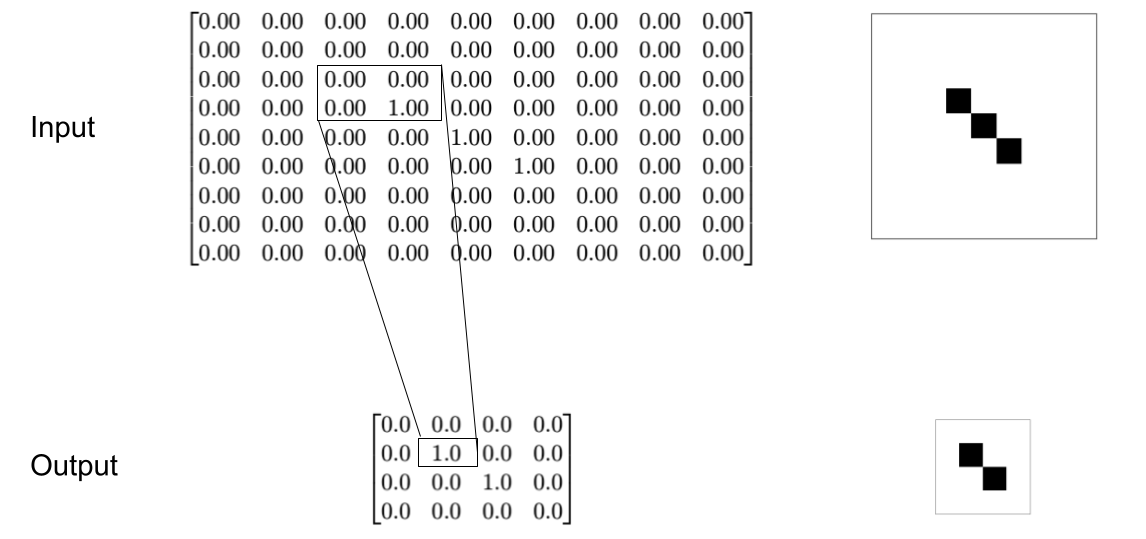
\includegraphics[scale=.3]{./images/maxPooling.png}
\caption[Jeff Yoshimi ]{Max pooling operation being applied to a matrix input, producing a smaller output that retains the same core information. The operator is shown by a square which shows the pool size. In this example the stride is 2, so it is scanned across the input in increments of 2. The maximum value in the pool is used to populate the output as the window is scanned across. Note that there is no depth here. Pooling operations are generally applied to 2d arrays.}
\label{maxPooling}
\end{figure}

A \glossary{pooling layer} is useful when tensors start getting too big. The idea is to go from bigger to smaller tensors, to keep these more computationally manageable. But we must do it in a way that preserves important information. Here again we pass a window over the input and slide it left-to-right and top-to-bottom, but instead of multiplying or dotting, we just take an average or a max value. The output is then a smaller tensor. 

There are two common pooling operations:

\begin{description}
\item[Max pooling] In each window, the maximum number is taken and written to an output matrix.
\item[Average pooling] The average value across a window is written to an output matrix.
\end{description}

These are sometimes called subsampling or downsampling methods. They are valuable in that they reduce the overall size of the network while preserving important structures.

The window passed over the input volume has a pool size, a width and height. It does not usually have depth because we do not want to combine the results of several feature maps. We pass the pooling operation over every feature map separately. The idea comes from the last section, where we saw that each filter learns to represent the inputs in a new way. When we downsample, we don't want to lose those differences. However, a new convolutional layer can learn to combine information.

However we can use a stride when we downsample. So the formula is the same as above when computing output shape from input shape.

An example is shown in figure \ref{maxPooling}. The pool is $2 x 2$ and the stride is $2$, so the window is passed over the input 2 at a time (notice that the right-most column gets left out in this case; a stride of 1 would fix that, or some padding). 

For these operations we use the same equations as above, but with pool width and height. There is no depth because pooling does not pool across channels.

\begin{align*}
\text{Output Width} &= \left( \frac{\text{Input Width} - \text{Pool Window Width}}{\text{Pool Stride}} \right) + 1 \\
\text{Output Height} &= \left( \frac{\text{Input Height} - \text{Pool Window Height}}{\text{Pool Stride}} \right) + 1
\end{align*} 

\subsection{Flattening and Dense Layers}

Another thing we can do, usually in the final layers of a deep CNN, is to ``flatten'' a volume back into a vector, converting the tensor into a node layer, and thus taking us back to the world of traditional neural networks focused on in much of the book. If we have a 5x5 this becomes the activation vector for a node layer with 25 nodes. If we have a 4x5x10 this becomes the activation vector for a node layer with 200 nodes. Then we just do things as we've done before.

These layers are conventional fully-connected dense layers. 

The overall idea is to start with layers that learn these complex features, then to compress these representations with subsampling, and finally to present the results to the final layers, which are basically familiar backprop networks presented with the results of a whole lot of convolving and subsampling. 

\begin{figure}[h]
\centering
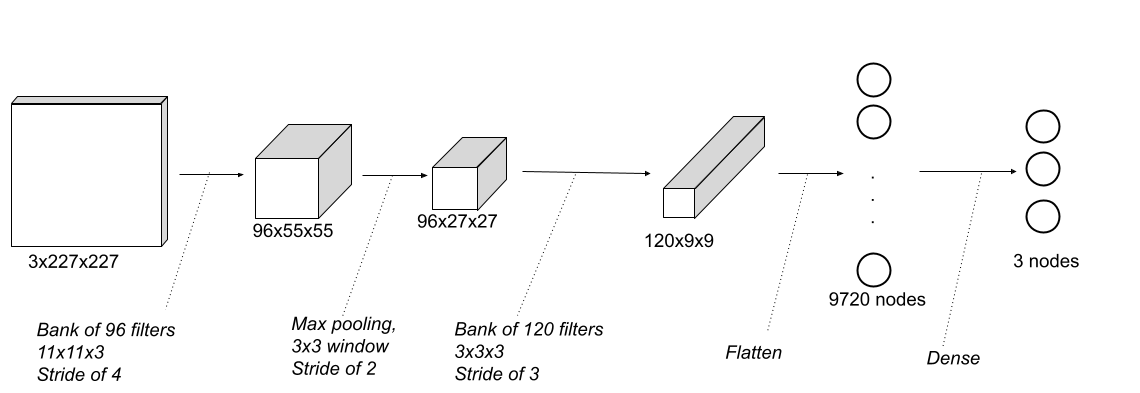
\includegraphics[scale=.45]{./images/deepNetExample.png}
\caption[Soraya Boza and Jeff Yoshimi ]{Sample deep network showing convolutional layers and pooling layers. You should try applying the shape equations to convince yourself that the sizes make sense. }
\label{deepNetExample}
\end{figure}


\section{Applications of Convolutional Networks}

% This section obviously needs to be developed
% What do convolutional layers correspond to in the brain?
 
As discussed in section \extref{deep_revolution}, deep networks and deep learning led to a revolution in neural networks beginning in the 2010s. The revolution was in engineering initially, but the history of deep networks shows that they have applications across all the domains of neural network research: engineering, computational neuroscience, connectionism, and computational cognitive neuroscience. 

Deep network models originate in  computational neuroscience models of vision that were developed in the 1970s and 1980s \cite{fukushima1982neocognitron}. These ideas were later used to engineer pattern recognition networks. A famous early application was recognizing zip codes written on envelopes \cite{lecun1989backpropagation}. As deep networks became mainstream based on technical improvements (big data, GPU and hardware acceleration, better architectures and training algorithms), scientists began using them, for example, to model the response profile of neurons in the visual system (recall the discussion of figure \extref{deepLearning_Vision} in chapter \extref{ch_neuro}). 

The idea is also relevant to connectionism and computational cognitive neuroscience. Recall from the history chapter that the concept of layered feature detection goes back to Oliver Selfridge and his ``pandemonium'' model, which at the time just speculated that in seeing letters a hierarchy of ``demons'' pass messages along: from edge demons to curve edges and finally to the output layer's ``B demon'' (see figure \extref{selfridge} in chapter \extref{ch_history}). Deep networks instantiate this idea, in such a way that we can actually  see what their receptive fields are.\footnote{The receptive fields can be quite strange and even disturbing. See \url{https://distill.pub/2017/feature-visualization/} for some striking demonstrations.}  The significance of these networks for psychology is still in its infancy, but early results are promising \cite{zorzi2013modeling, ritter2017cognitive}.
% Work more on interpreting what is happening in that distll article, and add some material here, including pictures of the weird features. Then add some colab demos to the course.
